
\section{Directed graph fuel cycle analysis and \Cyclus}
\subsection{Acquisition Pathway Analysis (APA)}

\begin{frame}{Motivation}
\begin{block}{Acquisition Pathway Analysis (APA)} Assess technically plausible steps a State could take to acquire material that could be used in a nuclear explosive device \cite{amano_conceptualization_2013}
\end{block}
  \begin{itemize}
  \medskip
  %\item Enhance state evaluation capabilities (IAEA R\&D objective V.2.R1)
    \item Objective and reproducible analysis for any set of fuel cycle facilities and capabilities
  \item Bring experience in modeling nuclear material flows to the nonproliferation and safeguards community
    \bigskip
    \begin{figure}
        \centering
        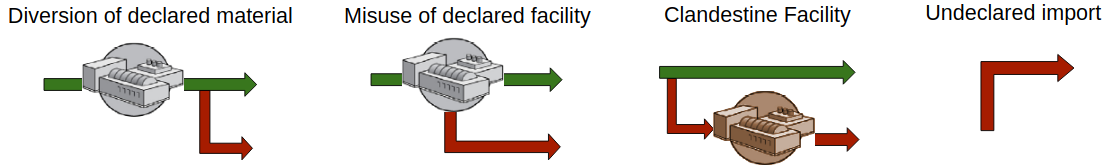
\includegraphics[width=0.95\linewidth]{images/path_step_types.png}
        \caption{Four path steps to capture, based on \cite{renis_conducting_2014}}
        \label{fig:path_steps}
    \end{figure}

  \end{itemize}

\end{frame}


\subsection{\Trailmap}
% ---------------------------------------------- %
\begin{frame}{Introducing \Trailmap}
    \begin{columns}
     \column{0.55\textwidth}
     \begin{itemize}
         \item \Trailmap is a new Cyclus module to conduct APA
     \end{itemize}
     \bigskip
    Before running \Trailmap
    \begin{itemize}
        \item User gathers State-specific factors and information
        \item Creates a \Cyclus input file with the set of existing facilities as well as technologically feasible undeclared activities and facilities
    \end{itemize}
    \column{0.45\textwidth}
    \begin{figure}
        \centering
        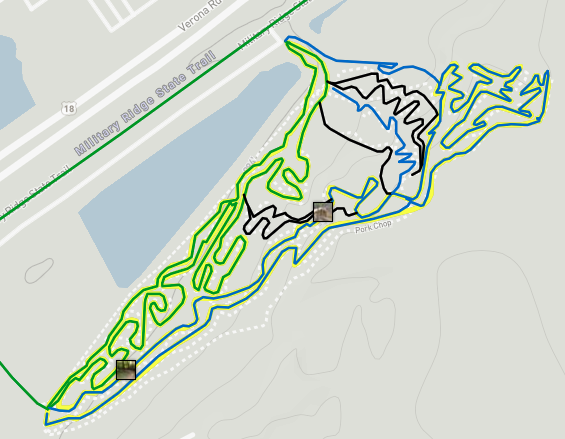
\includegraphics[width=0.85\textwidth]{images/Trailmap.png}
        \caption{From MTB Project}
        \label{fig:mtb}
    \end{figure}
    \end{columns}
    \bigskip
   Trailmap is also open-source and is available at \href{https://github.com/cnerg/trailmap}{https://github.com/cnerg/trailmap}
\end{frame}
% ---------------------------------------------- %

% ---------------------------------------------- %
\begin{frame}{\Trailmap}

    \begin{enumerate}
        \item Identify installed \Cyclus modules
        \item Reads in \Cyclus input file, identifying agents and commodities
        \item Builds a directed graph $G = (V, \ E)$ of facilities and commodities using NetworkX
        \item Depth-first search from all sources to all sinks
        \item Visualize graph using Jupyter notebook
        \item Filter and sort pathways using analysis tools
        \item Run Cyclus for individual path or groups of paths
    \end{enumerate}
    \color{gray}{\small{Future work}}
    \begin{enumerate}
        \setcounter{enumi}{6}
        {\setbeamercolor{enumerate item}{fg=gray}\color{gray}
        \item Further sorting and filtering of pathways based on throughput
        \item Test notional safeguards}
    \end{enumerate}
\end{frame}
% ---------------------------------------------- %


\subsection{\Trailmap Demonstration}
% ---------------------------------------------- %
\begin{frame}{Example "Republic of Bundy"}
    \begin{columns}
    \column{0.53\textwidth}
    \begin{figure}
        \centering
        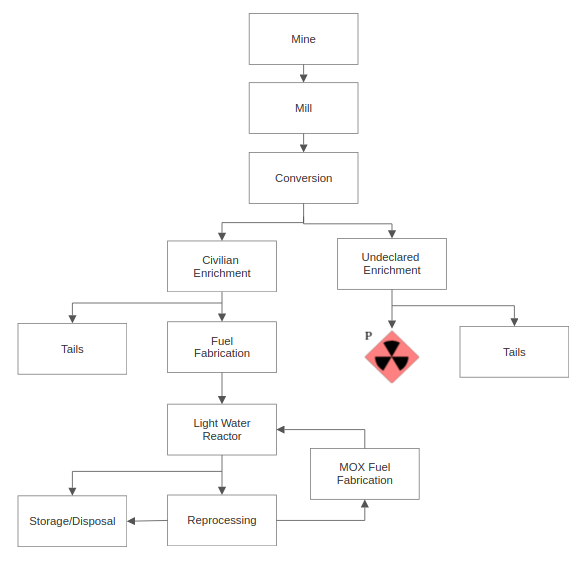
\includegraphics[width=\textwidth]{images/example.png}
        \caption{Network flow of "ROB" fuel cycle}
        \label{fig:ROB}
    \end{figure}
    \column{0.42\textwidth}
    \begin{itemize}
        \item Small but well-developed fuel cycle
        \item Civilian declared enrichment and reprocessing
        \item Clandestine enrichment facility
    \end{itemize}
    \begin{figure}[h]
        \centering
        
\includegraphics[width=0.8\linewidth]{images/Bundy.jpg}
        \caption{\small Former foster dog Bundy}
        \label{fig:my_label}
    \end{figure}
    \end{columns}
\end{frame}
% ---------------------------------------------- %

% ---------------------------------------------- %
\begin{frame}{Pathways}
    \begin{itemize}
        \item Mine, Mill, Conversion, Declared Enrichment, Tails
        \item Mine, Mill, Conversion, Undeclared Enrichment, HEU/Pu
        \item Mine, Mill, Conversion, Declared Enrichment, Fuel Fab, LWR, Waste Storage, Reprocessing, MOX Fuel Fab, HEU/Pu
        \item Mine, Mill, Conversion, Declared Enrichment, Fuel Fab, LWR, Reprocessing, MOX Fuel Fab, HEU/Pu
        \item Mine, Mill, Conversion, Declared Enrichment, Fuel Fab, LWR, Reprocessing, HEU/Pu
        \item Mine, Mill, Conversion, Declared Enrichment, Undeclared Enrichment, HEU/Pu
        \item Mine, Mill, Conversion, Declared Enrichment, Fuel Fab, LWR, Waste Storage, Reprocessing, HEU/Pu
        \item Mine, Mill, Conversion, Declared Enrichment, HEU/Pu
        \item Mine, Mill, Conversion' Declared Enrichment, Undeclared Enrichment, Undeclared Tails,
        \item Mine, Mill, Conversion, Declared Enrichment, Undeclared Tails
    \end{itemize}
\end{frame}
% ---------------------------------------------- %

% ---------------------------------------------- %
\begin{frame}{Acquisition Paths}
    \begin{itemize}
        \item \st{Mine, Mill, Conversion, Declared Enrichment, Tails}
        \item Mine, Mill, Conversion, Undeclared Enrichment, HEU/Pu
        \item Mine, Mill, Conversion, Declared Enrichment, Fuel Fab, LWR, Waste Storage, Reprocessing, MOX Fuel Fab, HEU/Pu
        \item Mine, Mill, Conversion, Declared Enrichment, Fuel Fab, LWR, Reprocessing, MOX Fuel Fab, HEU/Pu
        \item Mine, Mill, Conversion, Declared Enrichment, Fuel Fab, LWR, Reprocessing, HEU/Pu
        \item Mine, Mill, Conversion, Declared Enrichment, Undeclared Enrichment, HEU/Pu
        \item Mine, Mill, Conversion, Declared Enrichment, Fuel Fab, LWR, Waste Storage, Reprocessing, HEU/Pu
        \item Mine, Mill, Conversion, Declared Enrichment, HEU/Pu
        \item \st{Mine, Mill, Conversion' Declared Enrichment, Undeclared Enrichment, Undeclared Tails}
        \item \st{Mine, Mill, Conversion, Declared Enrichment, Undeclared Tails}
    \end{itemize}
\end{frame}
% ---------------------------------------------- %


% ---------------------------------------------- %
\begin{frame}{Visualizing}
    \begin{itemize}
        \item Automated interactive visualization using Jupyter Notebooks and Plotly package
        \item Graphviz 'dot' to layout nodes
        \begin{itemize}
            \item Good starting point, designed for trees
            \item NFC are not quite trees, but almost
        \end{itemize}
    \end{itemize}
    \begin{figure}
        \centering
        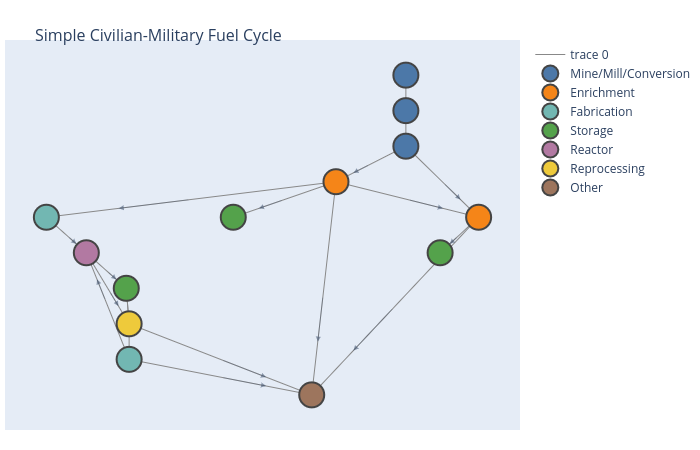
\includegraphics[width=0.75\textwidth]{images/newplot.png}
        \label{fig:example_viz}
    \end{figure}
\end{frame}
% ---------------------------------------------- %


% ---------------------------------------------- %
\begin{frame}{Facility-specific pathways: reprocessing}
    \begin{itemize}
        \item \st{Mine, Mill, Conversion, Declared Enrichment, Tails}
        \item Mine, Mill, Conversion, Undeclared Enrichment, HEU/Pu
        \item \textbf{Mine, Mill, Conversion, Declared Enrichment, Fuel Fab, LWR, Waste Storage, Reprocessing, MOX Fuel Fab, HEU/Pu}
        \item \textbf{Mine, Mill, Conversion, Declared Enrichment, Fuel Fab, LWR, Reprocessing, MOX Fuel Fab, HEU/Pu}
        \item \textbf{Mine, Mill, Conversion, Declared Enrichment, Fuel Fab, LWR, Reprocessing, HEU/Pu}
        \item Mine, Mill, Conversion, Declared Enrichment, Undeclared Enrichment, HEU/Pu
        \item \textbf{Mine, Mill, Conversion, Declared Enrichment, Fuel Fab, LWR, Waste Storage, Reprocessing, HEU/Pu}
        \item Mine, Mill, Conversion, Declared Enrichment, HEU/Pu
        \item \st{Mine, Mill, Conversion' Declared Enrichment, Undeclared Enrichment, Undeclared Tails}
        \item \st{Mine, Mill, Conversion, Declared Enrichment, Undeclared Tails}
    \end{itemize}
\end{frame}
% ---------------------------------------------- %

% ---------------------------------------------- %
\begin{frame}{Shortest pathways}
    \begin{itemize}
        \item \st{Mine, Mill, Conversion, Declared Enrichment, Tails}
        \item \textcolor{red}{Mine, Mill, Conversion, Undeclared Enrichment, HEU/Pu}
        \item Mine, Mill, Conversion, Declared Enrichment, Fuel Fab, LWR, Waste Storage, Reprocessing, MOX Fuel Fab, HEU/Pu
        \item Mine, Mill, Conversion, Declared Enrichment, Fuel Fab, LWR, Reprocessing, MOX Fuel Fab, HEU/Pu
        \item Mine, Mill, Conversion, Declared Enrichment, Fuel Fab, LWR, Reprocessing, HEU/Pu
        \item Mine, Mill, Conversion, Declared Enrichment, Undeclared Enrichment, HEU/Pu
        \item Mine, Mill, Conversion, Declared Enrichment, Fuel Fab, LWR, Waste Storage, Reprocessing, HEU/Pu
        \item \textcolor{red}{Mine, Mill, Conversion, Declared Enrichment, HEU/Pu}
        \item \st{Mine, Mill, Conversion' Declared Enrichment, Undeclared Enrichment, Undeclared Tails}
        \item \st{Mine, Mill, Conversion, Declared Enrichment, Undeclared Tails}
    \end{itemize}
\end{frame}
% ---------------------------------------------- %


% ---------------------------------------------- %
\begin{frame}{Other Tools}
    \begin{itemize}
        \item Search over a given list of facilities
        \begin{itemize}
            \item Pathways that contain \textit{any} facilities in the list
            \item Pathways that contain \textit{all} facilities in the list
        \end{itemize}
        \item Pathways that flow between a specific source and/or target node        \begin{itemize}
            \item Node disjoint paths
        \end{itemize}
        \item Cyclical or looping pathways (reprocessing)
        \item Graph parameters
        \begin{itemize}
            \item Graph semiconnectedness
            \item Flow hierarchy
            \item Shortest, longest paths
        \end{itemize}
        \item Flow (throughput)
        \begin{itemize}
            \item Flow of a given pathway
            \item Maximum total flow (complete breakout)
            \item Maximum flow pathway
            \item All pathways with flow above a threshold
        \end{itemize}
    \end{itemize}
\end{frame}
% ---------------------------------------------- %

\section{Conclusions \& Future Work}
% ---------------------------------------------- %
\begin{frame}{Conclusions}
    \begin{itemize}
        \item \Trailmap can conduct APA
        \item Basic interactive visualization is running
        \item \Trailmap is mostly a command-line tool right now, but can also be used from a Jupyter Notebook
        \item Next up: 
        \begin{itemize}
            \item Automating import of throughput information from \Cyclus simulation into \Trailmap
            \item Calculating time to completion for paths of interest
            \item Revamp visualization tool
        \end{itemize}
    \end{itemize}
\end{frame}
% ---------------------------------------------- %

% ---------------------------------------------- %
\begin{frame}{Future Work}
    \begin{itemize}
        \item Capture time-dependent evolution of acquisition paths
        \item Evaluate user interface to \Trailmap
        \item Add MBAs to existing \Cyclus facilities and build notional safeguards
        \begin{itemize}
            \item Expand MBAs and signatures from recycle:Pyre archetype \cite{westphal_modeling_2019}
            \item Expand inspector swipes from mbmore:RandomEnrich\cite{mcgarry_mbmore_2018}
        \end{itemize}
    \end{itemize}
    \begin{figure}
        \centering
        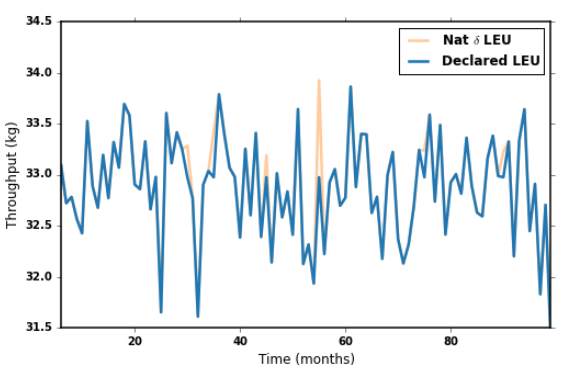
\includegraphics[width=0.3\textwidth]{images/Mcgarry_diversion.png}
        \caption{mbmore modeling of protracted diversion at an enrichment facility}
        \label{fig:McGarry_diversion}
    \end{figure}
\end{frame}
% ---------------------------------------------- %
